\section{Praxisbeispiel}\label{sec:praxisbeispiel}
Im Folgenden wird der Workflow mit \gls{dfl} näher betrachtet.
Anschließend werden verschiedenen Konfigurationen und Trainingsdauern verglichen.

\subsection{Laborumgebung}\label{subsec:laborumgebung}
Alle Deepfakes, wenn nicht anders genannt, werden auf folgender Hardware erstellt.\\[0.5cm]
\begin{tabular}{rl}
    CPU:& \texttt{AMD Ryzen 5 2600X}\\
    RAM:& \texttt{16GB DDR4 3000MHz}\\
    GPU:& \texttt{NVIDIA RTX 2070 (8GB GDDR6 VRAM)}\\
    OS:& \texttt{Windows 11}
\end{tabular}\\[0.5cm]

Ziel des Deepfakes ist das Gesicht von \gls{rdj} auf Prof. Volker Knoblauch in diesem \href{https://www.youtube.com/watch?v=rksMPlRSbQU}{Video} zu swappen,
sodass die Hochschule Aalen amerikanische Prominente auf ihrem Youtube-Kanal zeigen kann.

\subsection{Programmstruktur}\label{subsec:programmstruktur}
Nach der Installation von \gls{dfl} finden sich im entsprechenden Ordner eine Vielzahl von \texttt{.bat}-Dateien, sowie ein \texttt{\_internal}- und \texttt{workspace}-Ordner.
Die \texttt{.bat}-Dateien führen die im \texttt{\_internal}-Ordner abgelegten Scripte mit den entsprechenden Parametern aus.
Es wäre also möglich auf die Dateien zu verzichten und \gls{dfl} lediglich über eine Konsole auszuführen.
Alle Dateien, die während der Erstellung eines Deepfakes erstellt oder benötigt werden, werden im \texttt{workspace}-Ordner abgelegt.
Bei der Installation von \gls{dfl} werden Beispieldaten mit geladen.\\

Immer wieder finden sich die Bezeichnungen \texttt{src} und \texttt{dst}.
Diese referenzieren in \gls{dfl}:
\begin{itemize}
    \item \textbf{src (Source):} Das Gesicht, bzw. das zugehörige Videomaterial, das über das Zielgesicht gelegt werden soll.
    \item \textbf{dst (Destination):} Das Gesicht, bzw. das zugehöhrige Videomaterial, das ersetzt werden soll.
\end{itemize}

\subsection{Vorbereitung}\label{subsec:vorbereitung}
Bevor ein Deepfake erstellt werden kann, muss zuerst einmal geeignetes Ausgangsmaterial gesammelt werden.
Generell gilt, je besser das Trainingsmaterial, desto besser werden die Deepfakes.
Die Qualität des Ausgangsmaterials hängt von der Auflösung, der Belichtung, der Vielseitigkeit der Ausdrücke und der verschiedenen Aufnahmewinkeln (Fig. \ref{fig:head-angles-diagram}) ab.
Dabei gilt, je ähnlicher Source- und Destination-Material sind, desto überzeugender wird das Ergebnis.
\begin{figure}
    \center
    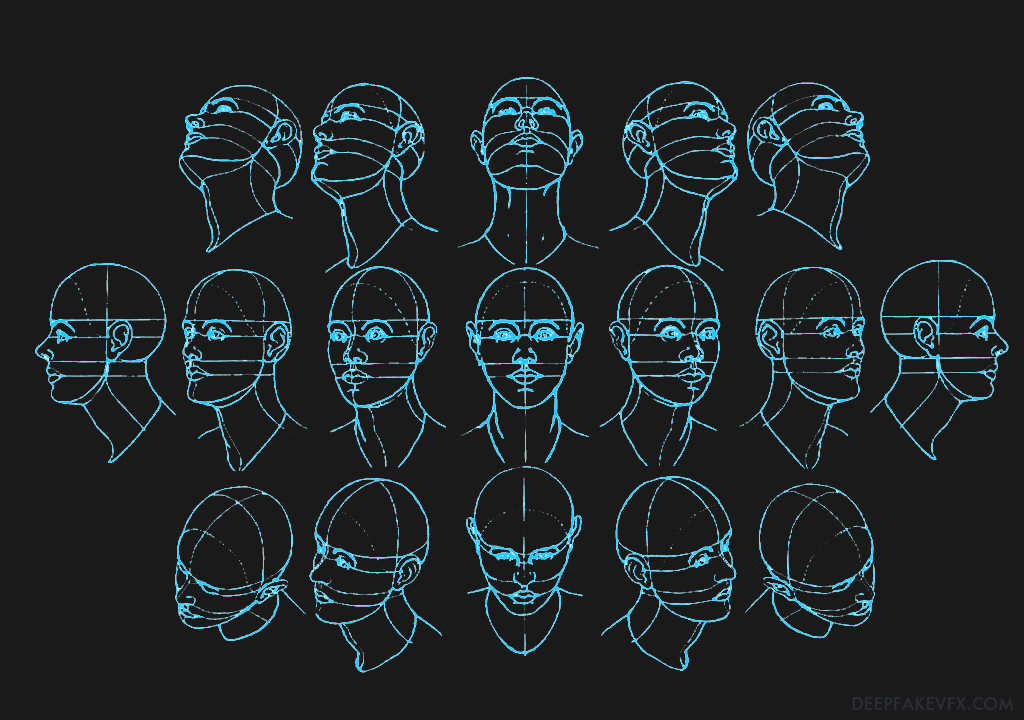
\includegraphics[width=0.5\textwidth]{Bilder/DFL/Human_Head_Angles_Diagram}
    \caption{Head Angles Diagram}
    \label{fig:head-angles-diagram}
\end{figure}

Ein Trainingsdatensatz sollte mehrere Hundert Bilder umfassen.
Je nach Resolution des trainierten Models sollten die Zahlen sogar in die Tausende gehen.\\[0.5cm]

Für den exemplarischen Deepfake dieser Arbeit, werden das mitgelieferte Standardvideo von \gls{rdj} als \texttt{Source} und das Interview von Prof. Dr. Harald Rieger und Prof. Volker Knoblauch als \texttt{Destination} verwendet.

\subsection{Pretraining}\label{subsec:pretraining}
Wie in \ref{subsubsec:pretraining} beschrieben wird ein vortrainiertes Modell verwendet.
\gls{dfl} liefert bereits einen Datensatz zum Vortrainieren mit.
Das Pretraining kann also ohne weitere Vorbereitung beginnen.
\subsubsection{Pretrain XSeg}
\begin{lstlisting}[label={lst:xseg-pretraining},numbers=none]
    5.XSeg) train.bat
\end{lstlisting}
Öffnet die Konsole für die Konfiguration.
\begin{itemize}
    \item \textbf{Face type:} Bestimmt wie viel von einem Gesicht ersetzt werden soll. Z.B. das Gesicht mit oder ohne Stirn usw.
    \item \textbf{Batch\_size:} Je höher die Batch size, desto größer die Hardwareanforderungen und desto besser die Ergebnisse
    \item \textbf{Enable pretraining mode:} Selbsterklärend
\end{itemize}
Nach einem Test ob die Hardware ausreichend für die Konfiguration ist, startet das Training (Abbildung \ref{fig:xseg-pretrain}).
\begin{figure}
    \center
    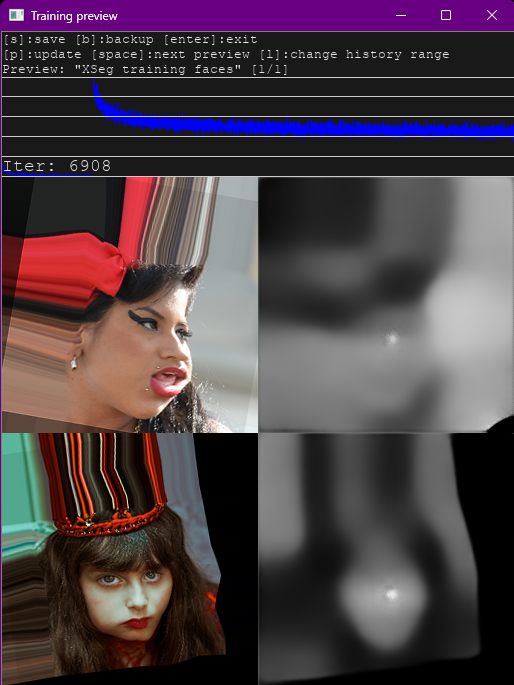
\includegraphics[width=0.7\textwidth]{Bilder/DFL/XSegEditor-3-pretrain}
    \caption{XSeg Pretraining im \textit{head} Modus}
    \label{fig:xseg-pretrain}
\end{figure}

\subsubsection{Pretrain SAEHD}
\begin{lstlisting}[label={lst:saehd-pretraining},numbers=none]
    6) train SAEHD.bat
\end{lstlisting}
Dies öffnet die Konsole um ein neues Modell zu konfigurieren.
Für das Pretraining können alle Einstellungen, außer wenige Ausnahmen, auf Standard gelassen werden.
Geändert werden sollten die Folgenden:
\begin{itemize}
    \item \textbf{Autobackup every N hour:} Selbsterklärend
    \item \textbf{Target iteration:} Sinnvolle Werte für Pretraining sind 500 Tausend bis 1 Million
    \item \textbf{Resolution:} Je höher der Wert, desto hochaufgelöster das Ergebnis. Für \texttt{face} und \texttt{whole-face} sind $128$ ausreichend. Für \texttt{head} mindestens $224$. Für das bestmögliche Ergebnis so hoch setzten wie die Hardware mithalten kann.
    \item \textbf{Face type:} Bestimmt wie viel von einem Gesicht ersetzt werden soll. Z.B. das Gesicht mit oder ohne Stirn usw.
    \item \textbf{Batch\_size:} Analog zu Resolution. Nachdem sich für eine Resolution entschieden wurde, so hoch setzten bis die Hardware ausgelastet ist.
    \item \textbf{Enable pretraining mode:} Selbsterklärend
\end{itemize}
Nun wird ebenfalls die Hardware getestet und das Training gestartet (Abbildung \ref{fig:saehd-pretrain}).
\begin{figure}
    \center
    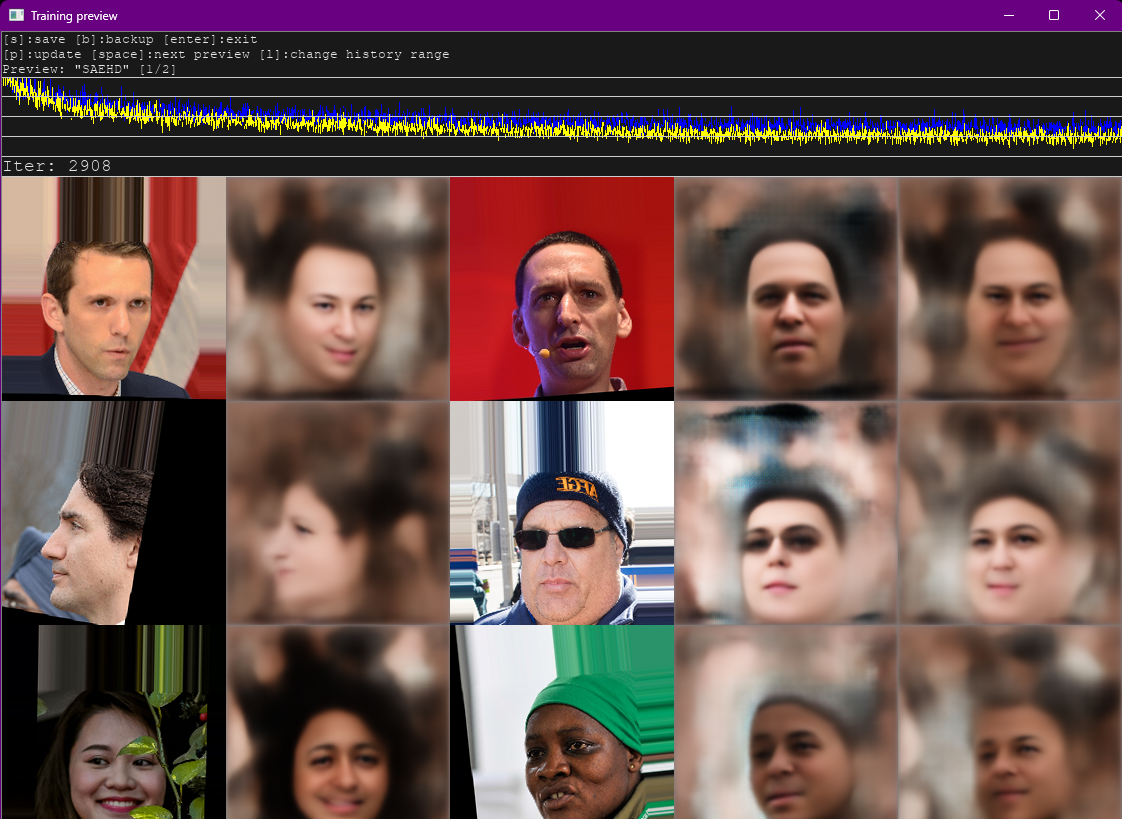
\includegraphics[width=0.7\textwidth]{Bilder/DFL/saehd-pretrain-head}
    \caption{SAEHD Pretraining mit 224 Resolution im \textit{head} Modus}
    \label{fig:saehd-pretrain}
\end{figure}

\subsection{Extraction}\label{subsec:extraction}
Im ersten Schritt werden die Videos zu einem Trainingsdatensatz verarbeitet.
\begin{lstlisting}[label={lst:extraction-1},numbers=none]
    2) extract images from video data_src.bat
    3) extract images from video data_dst FULL FPS.bat
\end{lstlisting}
Diese Skripts zerlegen mithilfe von FFmpeg das \texttt{src}- bzw. \texttt{dst}-Video in ihre einzelnen Frames.
Diese sind im \texttt{workspace} unter \texttt{data\_src} bzw. \texttt{data\_dst} zu finden.
Bei dem \texttt{src}-Video kann in der Konsole zusätzlich angegeben werden wie viele \gls{fps} extrahiert werden sollen.
Bei langen \texttt{src}-Videos kann dies sinnvoll sein.
Werden 5 \gls{fps} aus einem 4-minütigen Video extrahiert, ist die Variation der Bilder größer als 10 \gls{fps} aus einem 2-minütigen Video.
Natürlich können immer auch alle Frames extrahiert werden, hier muss der größere Speicheraufwand und die längere Trainingsdauer abgewogen werden.
Da das exemplarische Video gerade einmal $655$ Frames lang ist, können unbedenklich alle Frames genutzt werden.
Des Weiteren kann zwischen \texttt{PNG} und \texttt{JPG} entschieden werden.
Die Entscheidung bringt die üblichen Vor- und Nachteile der beiden Formate.
\begin{itemize}
    \item \textbf{PNG:} Verlustfreie Komprimierung \rightarrow Größere Dateien \rightarrow Kein Qualitätsverlust
    \item \textbf{JPG:} Verlustbehaftete Komprimierung \rightarrow Kleinere Dateien \rightarrow Qualitätsverlust
\end{itemize}
Da Speicherplatz für Videos dieser Länge nicht der entscheidende Faktor ist, kann hier die höhere Qualität von\texttt{PNG} genutzt werden.\\
Das \texttt{dst}-Video wird immer komplett extrahiert, da die Frames am Ende der Pipeline wieder zu einem Video zusammengesetzt werden.
Es müssen Frames vorhanden sein, um ein flüssiges Endergebnis zu gewährleisten.
Es kann ebenfalls das Bildformat ausgewählt werden, dieses sollte gleich gewählt werden wie beim ersten Video.\\[0.5cm]

Nun müssen die Gesichter aus den Bildern extrahiert werden.
Im Folgenden wird der Prozess für das \texttt{src}-Material (in \gls{dfl} Schritt 4.X) beschrieben.
Für das \texttt{dst}-Material verläuft der Prozess (als Schritt 5.X) analog.

Es gibt zwei Varianten die Gesichter aus den Frames zu extrahieren.
\begin{lstlisting}[numbers=none,label={lst:extraction-2}]
    4) data_src faceset extract MANUAL.bat
    4) data_src faceset extract.bat
\end{lstlisting}
Wie die Namen vermuten lassen werden die Gesichter einmal händisch und einmal durch ein vortrainiertes \gls{cnn} extrahiert.
Bei der automatischen Extraktion muss im Nachhinein ggf. falsch erkannte Gesichter manuell gelöscht werden.
Allerdings ist dieser Arbeitsaufwand bei weitem geringer als die manuelle Extraktion.
Bei der Ausführung können verschiedene Punkte konfiguriert werden.
Der \textbf{face type} gibt an wie viel vom Gesicht extrahiert werden soll.
\begin{itemize}
    \item \textbf{f (face):} Nur das Gesicht
    \item \textbf{wf (whole face):} Das ganze Gesicht inklusive Stirn und Kinn
    \item \textbf{h (head):} Der gesamte Kopf inklusive Haare
\end{itemize}
\textbf{Max numbers of faces} gibt an wie viele Gesichter pro Frame extrahiert werden sollen.
Dieser Wert sollte auf $0$ (alle) gesetzt werden.
Ist mehr als ein Gesicht in den Videos zu sehen, werden alle Gesichter extrahiert, nicht benötigte Bilder können anschließend wieder gelöscht werden.
Sind es zu viele Gesichter bzw. wird die Verarbeitungszeit zu hoch, muss entweder manuell oder mit einer Obergrenze extrahiert werden.
Im ersten Fall fällt erhöhter Arbeitsaufwand an, im zweiten Fall fällt der Datensatz kleiner aus, da das gewünschte Gesicht ggf. übersprungen wird.
Die Beispielvideos bestehen nur aus einem bzw. zwei Gesichtern und können unproblematisch automatisiert extrahiert werden.
Anschließend kann entweder im Standard Windows Explorer unter \texttt{workspace/data\_src/aligned} oder mithilfe des mitgelieferten Explorer die Daten gesichtet werden.
\begin{lstlisting}[label={lst:extraction-3},numbers=none]
    4.1) data_src view aligned result.bat
\end{lstlisting}
Dieses Skript öffnet den in Rust implementierten Explorer, welcher auf das schnelle Anzeigen von Bildern optimiert wurde.
\begin{figure}
    \center
    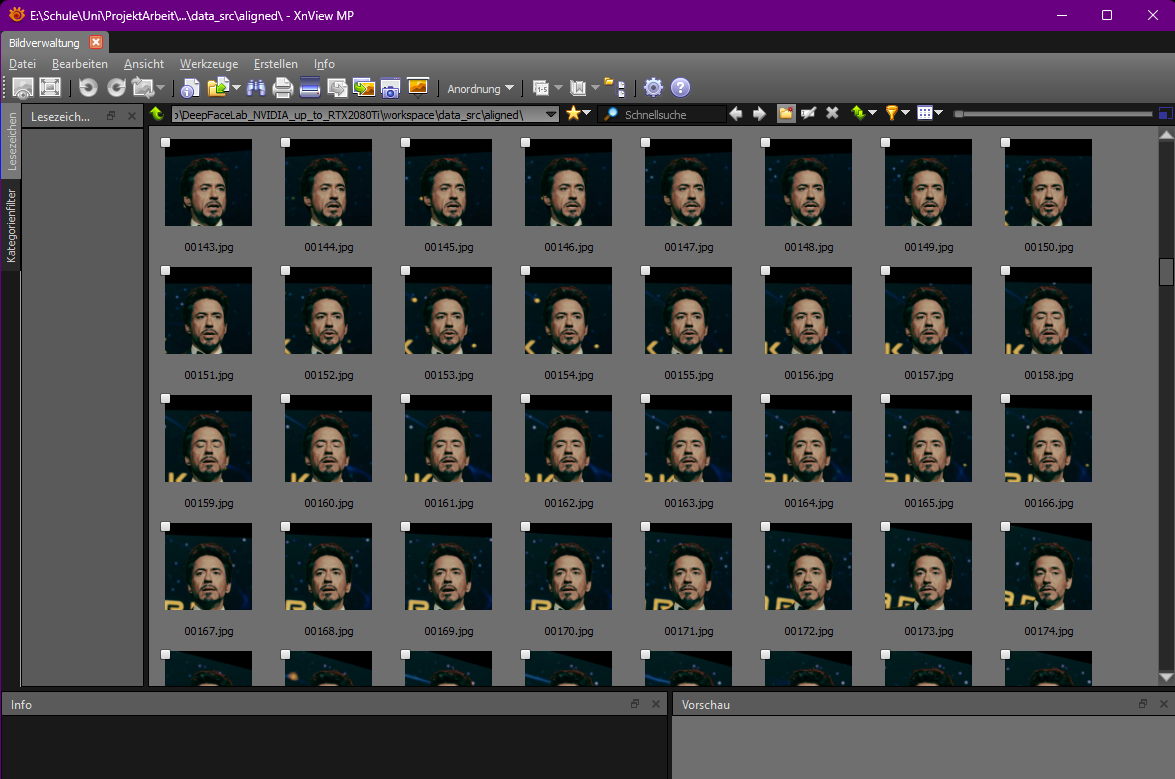
\includegraphics[width=0.7\textwidth]{Bilder/DFL/XnView}
    \caption{XnView (Rust Editor)}
    \label{fig:xnview}
\end{figure}
Nun müssen alle Bilder, die nicht richtig erkannt wurden gelöscht werden.
Dabei stellt \gls{dfl} einige Sortierungsmöglichkeiten zur Verfügung, die den Prozess erleichtern.
Diese sind zu einem Skript zusammengefasst.
\begin{lstlisting}[label={lst:extraction-4},numbers=none]
    4.2) data_src sort.bat
\end{lstlisting}
Durch das Sortieren nach \texttt{[0] blur} und \texttt{[1] motion\_blur} können schnell unscharfe Bilder ausfindig gemacht werden.
Durch die Sortierung nach \texttt{[5] histogram similarity} werden ähnliche Gesichter zusammen gruppiert.
So können Bilder einer nicht erwünschte zweiten Person einfach entfernt werden.\\
Ist die Auswahl der Gesichter abgeschlossen können diese noch bei Bedarf mit \gls{ai-upscaling} vergrößert werden.
Dies sollte nur gemacht werden, wenn die Bilder sonst unscharf oder zu klein sind.
Besser ist es direkt scharfe, hoch aufgelöste Bilder bzw. Ausgangsvideos zu verwenden.
Das Vorgehen ist für das \texttt{dst}-Material identisch.\\[0.5cm]

Sind alle Bilder entsprechend gesichtet und aussortiert, muss eine \texttt{XSeg Mask} angewandt werden.
Diese Maske erfasst das ganze Gesicht mit seinen genauen Umrissen.
Wenn Deepfakes im \textit{face} oder \textit{whole-face} Modus gemacht werden, kann eine pretrained generische Maske angewandt werden.
\begin{lstlisting}[label={lst:extraction-5},numbers=none]
    5.XSeg Generic) data_dst whole_face mask - apply.bat
    5.XSeg Generic) data_src whole_face mask - apply.bat
\end{lstlisting}
Für den \textit{head} Modus muss ein eigenes \texttt{XSeg-Model} trainiert werden.
Dafür werden mehrere Bilder benötigt, in die händisch der gewünschte Umriss gezeichnet wird.
Im Beispiel wäre das der gesamte Kopf, einschließlich Haaren.
\begin{lstlisting}[numbers=none,label={lst:extraction-6}]
    5.XSeg) data_dst mask - edit.bat
    5.XSeg) data_src mask - edit.bat
\end{lstlisting}
Diese Skripts öffnen den XSeg-Editor, indem die Polygone gezeichnet (Abbildung \ref{fig:xseg-editor-1}) werden können.
\begin{figure}
    \center
    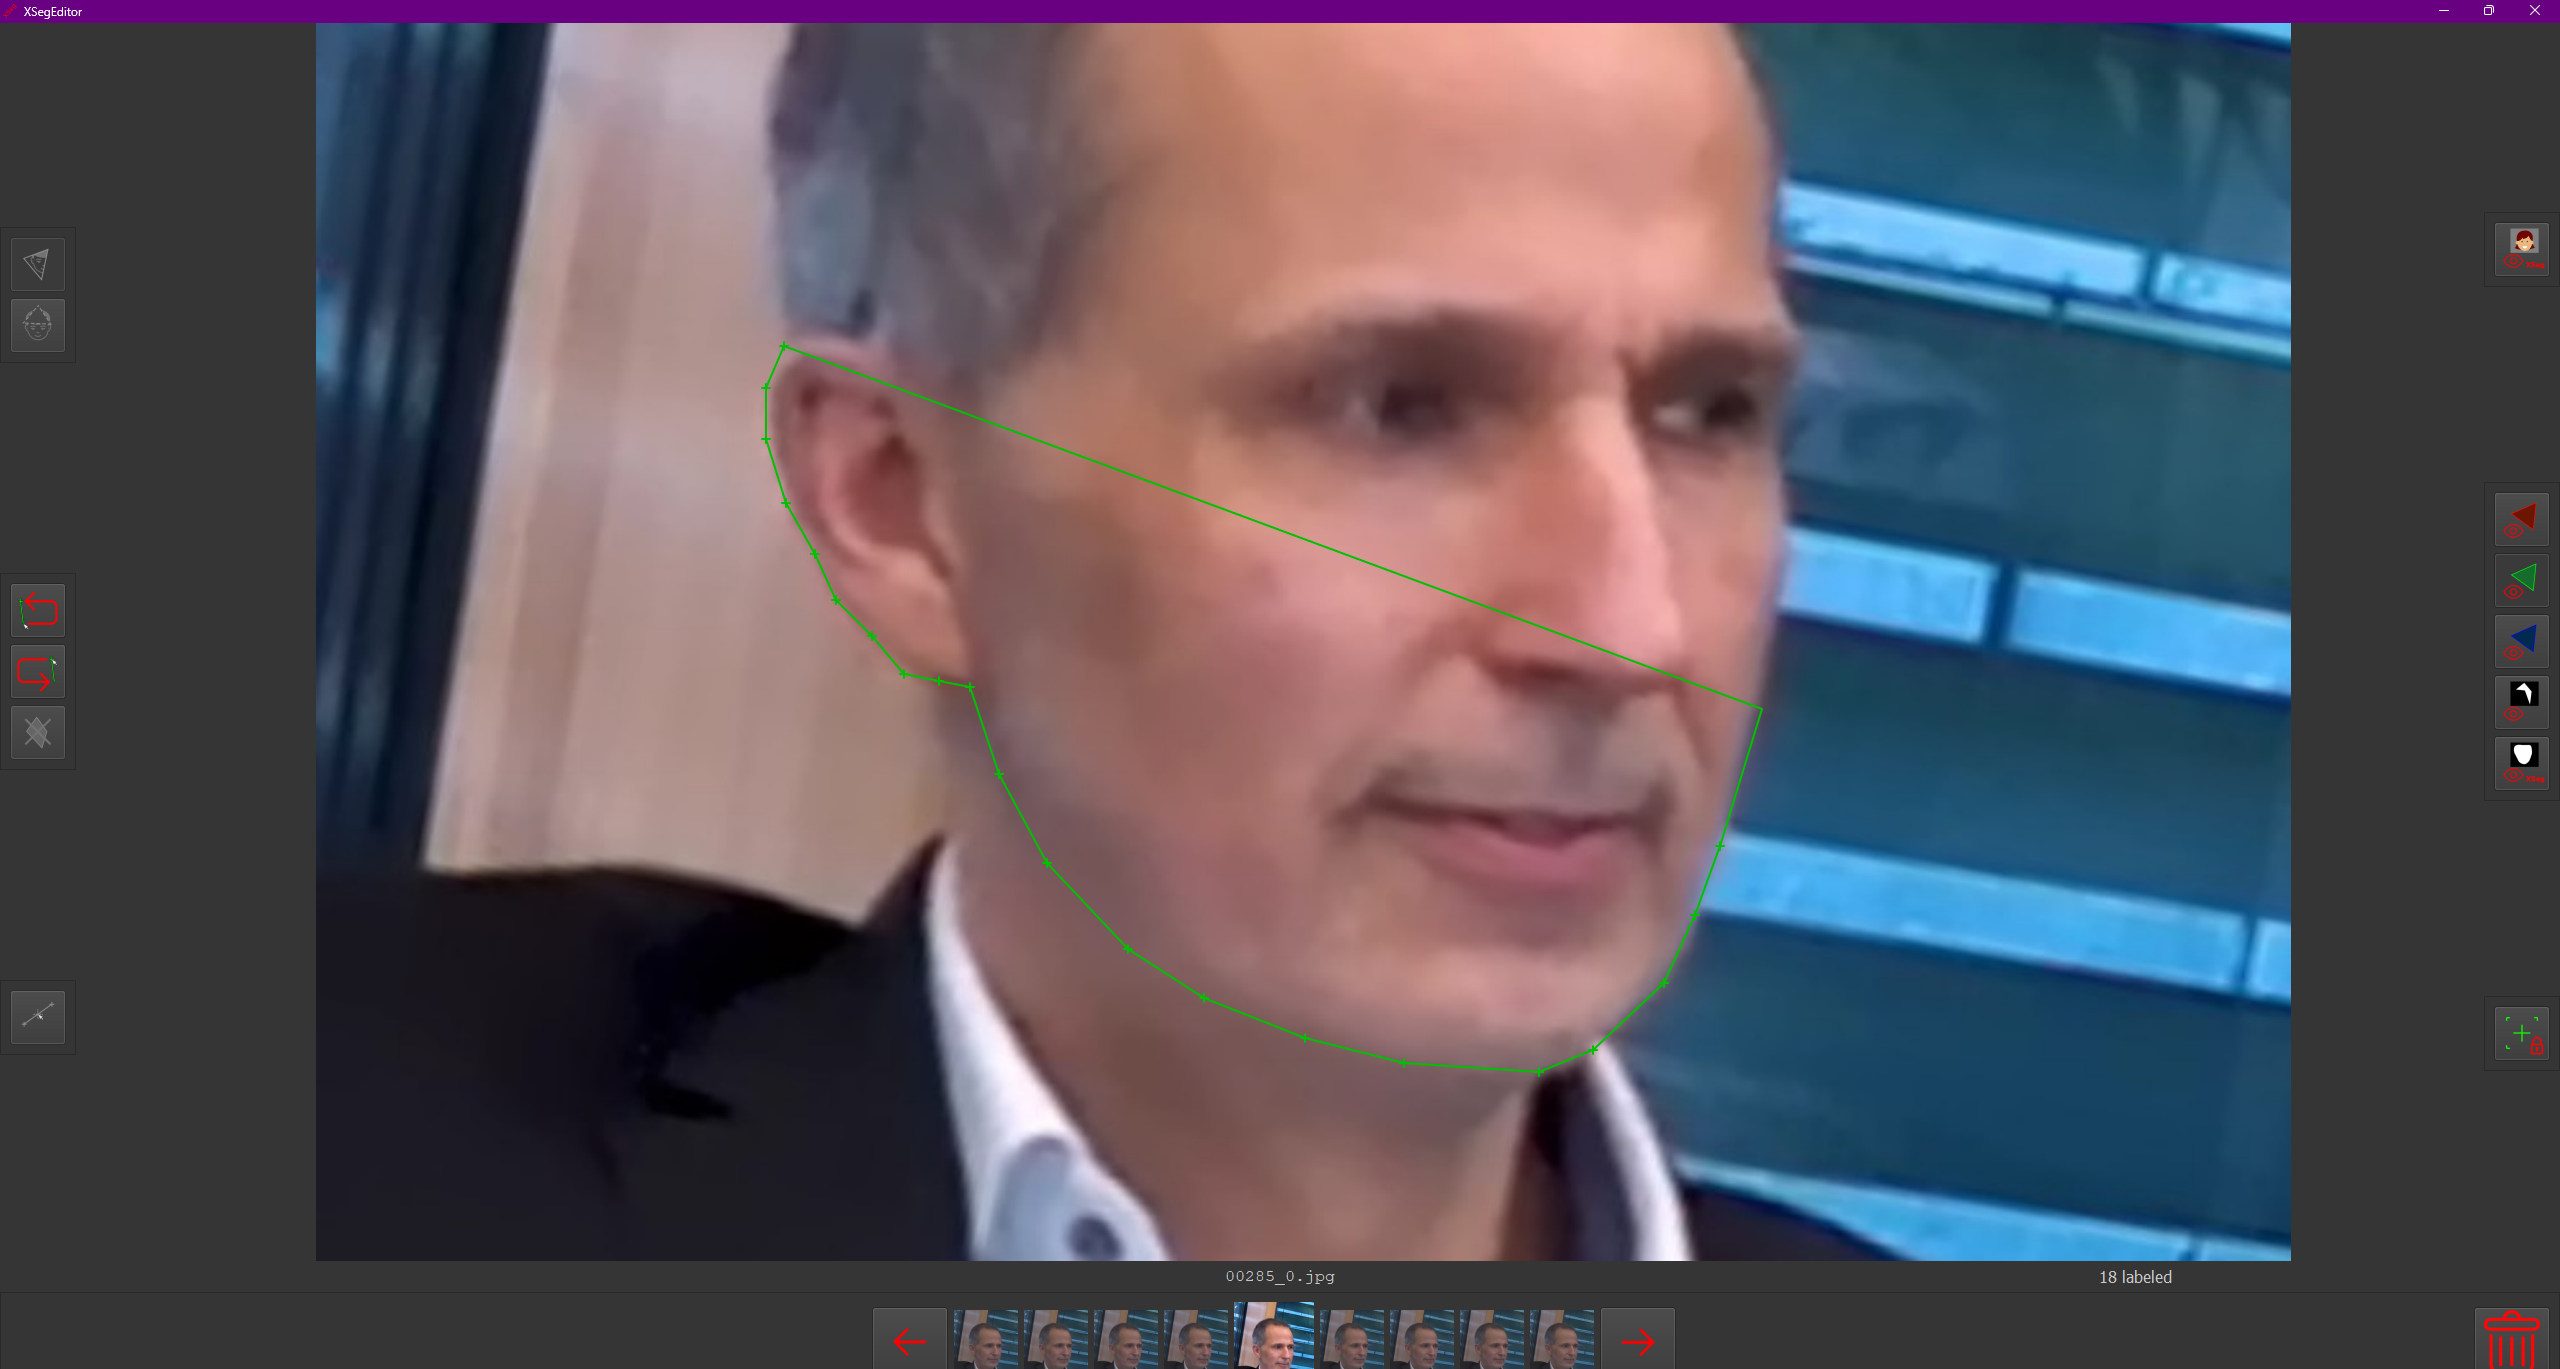
\includegraphics[width=0.7\textwidth]{Bilder/DFL/XSegEditor-1-draw}
    \caption{Polygon zeichnen im XSeg-Editor}
    \label{fig:xseg-editor-1}
\end{figure}
Es sollten je nach gewünschter Genauigkeit mehrere Dutzend bis wenige hundert Bilder markiert werden.
Wurde der Prozess für \texttt{src} und \texttt{dst} durchgeführt kann die Maske trainiert werden.
\begin{lstlisting}[label={lst:extraction-7},numbers=none]
    5.XSeg) train.bat
\end{lstlisting}
% TODO Maske trainieren und überprüfen
